

\chapter{Case study: interface design  |  案例研究:接口设计}
\label{turtlechap}

This chapter presents a case study that demonstrates a process for
designing functions that work together.

It introduces the {\tt turtle} module, which allows you to
create images using turtle graphics.  The {\tt turtle} module is
included in most Python installations, but if you are running Python
using PythonAnywhere, you won't be able to run the turtle examples (at
least you couldn't when I wrote this).

If you have already installed Python on your computer, you should
be able to run the examples.  Otherwise, now is a good time
to install.  I have posted instructions at
\url{http://tinyurl.com/thinkpython2e}.

Code examples from this chapter are available from
\url{http://thinkpython2.com/code/polygon.py}.

本章将通过一个案例研究,介绍如何设计出相互配合的函数。

本章会介绍 \lstinline{turtle} 模块,它可以让你使用海龟图形 (turtle graphics) 绘制图像。大部分的Python安装环境下都包含了这个模块,但是如果你是在 PythonAnywhere 上运行 Python 的,你将无法运行本章中的代码示例(至少在我写这章时是做不到的)。

如果你已经在自己的电脑上安装了 Python,那么不会有问题。如果没有,现在就是安装 Python 的好时机。我在 http://tinyurl.com/thinkpython2e 这个页面上发布了相关指南。

本章的示例代码可以从 http://thinkpython2.com/code/polygon.py 获得。

\section{The turtle module  |  turtle 模块}
\label{turtle}

To check whether you have the {\tt turtle} module, open the Python
interpreter and type

打开Python解释器,输入以下代码,检查你是否安装了 \lstinline{turltle} 模块:

\begin{lstlisting}
>>> import turtle
>>> bob = turtle.Turtle()
\end{lstlisting}

When you run this code, it should create a new window
with small arrow that represents the turtle.  Close the window.

上述代码运行后,应该会新建一个窗口,窗口中间有一个小箭头,代表的就是海龟。现在关闭窗口。

Create a file named {\tt mypolygon.py} and type in the following
code:

新建一个名叫  \lstinline{mypolygon.py} 的文件,输入以下代码:

\begin{lstlisting}
import turtle
bob = turtle.Turtle()
print(bob)
turtle.mainloop()
\end{lstlisting}


%
The {\tt turtle} module (with a lowercase 't') provides a function
called {\tt Turtle} (with an uppercase 'T') that creates a Turtle
object, which we assign to a variable named {\tt bob}.
Printing {\tt bob} displays something like:

\lstinline{turtle} 模块(小写的 \lstinline{'t'} )提供了一个叫作 \lstinline{Turtle} 的函数(大写的 \lstinline{'T'}),这个函数会创建一个 \lstinline{Turtle} 对象,我们将其赋值给名为 \lstinline{bob} 的变量。打印 \lstinline{bob} 的话,会输出下面这样的结果:

\begin{lstlisting}
<turtle.Turtle object at 0xb7bfbf4c>
\end{lstlisting}

%
This means that {\tt bob} refers to an object with type
{\tt Turtle}
as defined in module {\tt turtle}.

这意味着,\lstinline{bob} 指向一个类型为Turtle的对象,这个类型是由 \lstinline{turtle} 模块定义的。

\verb"mainloop" tells the window to wait for the user
to do something, although in this case there's not much for
the user to do except close the window.

\lstinline{mainloop} 告诉窗口等待用户操作,尽管在这个例子中,用户除了关闭窗口之外,并没有其他可做的事情。

Once you create a Turtle, you can call a {\bf method} to move it
around the window.  A method is similar to a function, but it
uses slightly different syntax.  For example, to move the turtle
forward:

创建了一个 \lstinline{Turtle} 对象之后,你可以调用 \emph{方法} (method) 来在窗口中移动该对象。方法与函数类似,但是其语法略有不同。例如,要让海龟向前走:

\begin{lstlisting}
bob.fd(100)
\end{lstlisting}

%
The method, {\tt fd}, is associated with the turtle
object we're calling {\tt bob}.
Calling a method is like making a request: you are asking {\tt bob}
to move forward.

方法 \lstinline{fd} 与我们称之为 \lstinline{bob} 的对象是相关联的。调用方法就像提出一个请求:你在请求 \lstinline{bob} 往前走。

The argument of {\tt fd} is a distance in pixels, so the actual
size depends on your display.


\lstinline{fd} 方法的实参是像素距离,所以实际前进的距离取决于你的屏幕。

Other methods you can call on a Turtle are {\tt bk} to move
backward, {\tt lt} for left turn, and {\tt rt} right turn.  The
argument for {\tt lt} and {\tt rt} is an angle in degrees.

\lstinline{Turtle} 对象中你能调用的其他方法还包括:让它向后走的 \lstinline{bk} ,向左转的 \lstinline{lt} ,向右转的 \lstinline{rt} 。 \lstinline{lt} 和 \lstinline{rt} 这两个方法接受的实参是角度。

Also, each Turtle is holding a pen, which is
either down or up; if the pen is down, the Turtle leaves
a trail when it moves.  The methods {\tt pu} and {\tt pd}
stand for ``pen up'' and ``pen down''.

另外,每个 \lstinline{Turtle} 都握着一支笔,不是落笔就是抬笔;如果落笔了, \lstinline{Turtle} 就会在移动时留下痕迹。 \lstinline{pu} 和 \lstinline{pd} 这两个方法分别代表``抬笔 (pen up)''和 ``落笔 (pen down)''。

To draw a right angle, add these lines to the program
(after creating {\tt bob} and before calling \verb"mainloop"):

如果要画一个直角 (right angle),请在程序中添加以下代码(放在创建 \lstinline{bob} 之后,调用 \lstinline{mainloop} 之前):

\begin{lstlisting}
bob.fd(100)
bob.lt(90)
bob.fd(100)
\end{lstlisting}

%
When you run this program, you should see {\tt bob} move east and then
north, leaving two line segments behind.

当你运行此程序时,你应该会看到 \lstinline{bob} 先朝东移动,然后向北移动,同时在身后留下两条线段 (line segment)。

Now modify the program to draw a square.  Don't go on until
you've got it working!

现在修改程序,画一个正方形。在没有成功之前,不要继续往下看。



%\newpage

\section{Simple repetition  |  简单重复}
\label{repetition}
\index{repetition}  \index{重复}

Chances are you wrote something like this:

很有可能你刚才写了像下面这样的一个程序:

\begin{lstlisting}
bob.fd(100)
bob.lt(90)

bob.fd(100)
bob.lt(90)

bob.fd(100)
bob.lt(90)

bob.fd(100)
\end{lstlisting}

%
We can do the same thing more concisely with a {\tt for} statement.
Add this example to {\tt mypolygon.py} and run it again:

我们可以利用一个 \lstinline{for} 语句,以更简洁的代码来做相同的事情。
将下面的示例代码加入 \lstinline{mypolygon.py} ,并重新运行:
\index{for loop}  \index{loop!for}  \index{statement!for}

\begin{lstlisting}
for i in range(4):
    print('Hello!')
\end{lstlisting}

%
You should see something like this:

你会看到以下输出:

\begin{lstlisting}
Hello!
Hello!
Hello!
Hello!
\end{lstlisting}

%
This is the simplest use of the {\tt for} statement; we will see
more later.  But that should be enough to let you rewrite your
square-drawing program.  Don't go on until you do.

这是 \lstinline{for} 语句最简单的用法;后面我们会介绍更多的用法。
但是这对于让你重写画正方形的程序已经足够了。 如果没有完成,请不要往下看。

Here is a {\tt for} statement that draws a square:

下面是一个画正方形的 \lstinline{for} 语句:

\begin{lstlisting}
for i in range(4):
    bob.fd(100)
    bob.lt(90)
\end{lstlisting}

%
The syntax of a {\tt for} statement is similar to a function
definition.  It has a header that ends with a colon and an indented
body.  The body can contain any number of statements.

for语句的语法和函数定义类似。
它有一个以冒号结尾的语句头(header)以及一个缩进的语句体(body)。
语句体可以包含任意条语句。

A {\tt for} statement is also called a {\bf loop} because
the flow of execution runs through the body and then loops back
to the top.  In this case, it runs the body four times.
\index{loop}

\lstinline{for} 语句有时也被称为 \emph{循环} (loop) ,因为执行流程会贯穿整个语句体,然后再循环回顶部。
在此例中,它将运行语句体四次。


This version is actually a little different from the previous
square-drawing code because it makes another turn after
drawing the last side of the square.  The extra turn takes
more time, but it simplifies the code if we do the same thing
every time through the loop.  This version also has the effect
of leaving the turtle back in the starting position, facing in
the starting direction.

这个版本事实上和前面画正方形的代码有所不同,因为它在画完正方形的最后一条边后,
又多转了一下。这个额外的转动多花了些时间,
但是如果我们每次都通过循环来做这件事情,这样反而是简化了代码。
这个版本还让海龟回到了初始位置,朝向也与出发时一致。



\section{Exercises  |  练习}

The following is a series of exercises using TurtleWorld.  They
are meant to be fun, but they have a point, too.  While you are
working on them, think about what the point is.

下面是一系列学习使用 \lstinline{Turtle} \footnote{译注:原文中使用的还是 \lstinline{TurtleWorld} ,应该是作者忘了修改。} 的练习。
这些练习也许很好玩,但它们是有针对性设计的。
在做这些练习的时候,可以思考一下它们的目的是什么。

The following sections have solutions to the exercises, so
don't look until you have finished (or at least tried).

后面几节是中介绍了这些练习的答案,因此如果你还没完成(或者至少试过),请不要看答案。

\begin{enumerate}

\item Write a function called {\tt square} that takes a parameter
named {\tt t}, which is a turtle.  It should use the turtle to draw
a square.

Write a function call that passes {\tt bob} as an argument to
{\tt square}, and then run the program again.

\item Add another parameter, named {\tt length}, to {\tt square}.
Modify the body so length of the sides is {\tt length}, and then
modify the function call to provide a second argument.  Run the
program again.  Test your program with a range of values for {\tt
length}.

\item Make a copy of {\tt square} and change the name to {\tt
  polygon}.  Add another parameter named {\tt n} and modify the body
  so it draws an n-sided regular polygon.  Hint: The exterior angles
  of an n-sided regular polygon are $360/n$ degrees.  \index{polygon
    function} \index{function!polygon}

\item Write a function called {\tt circle} that takes a turtle,
{\tt t}, and radius, {\tt r}, as parameters and that draws an
approximate circle by calling {\tt polygon} with an appropriate
length and number of sides.  Test your function with a range of values
of {\tt r}.  \index{circle function} \index{function!circle}

Hint: figure out the circumference of the circle and make sure that
{\tt length * n = circumference}.

\item Make a more general version of {\tt circle} called {\tt arc}
that takes an additional parameter {\tt angle}, which determines
what fraction of a circle to draw.  {\tt angle} is in units of
degrees, so when {\tt angle=360}, {\tt arc} should draw a complete
circle.
\index{arc function}
\index{function!arc}

\end{enumerate}

\begin{enumerate}

\item 写一个名为 \lstinline{square} 的函数,接受一个名为 \lstinline{t} 的形参, \lstinline {t} 是一个海龟。 这个函数应用这只海龟画一个正方形。

写一个函数调用,将 \lstinline{bob} 作为实参传给 \lstinline{square} ,然后再重新运行程序。

\item 给 \lstinline{square} 增加另一个名为 \lstinline{length} 的形参。
 修改函数体,使得正方形边的长度是 \lstinline{length} ,然后修改函数调用,提供第二个实参。
 重新运行程序。用一系列 \lstinline{length} 值测试你的程序。

\item 复制 \lstinline{square} ,并将函数改名为 \lstinline{polygon} 。
   增加另外一个名为 \lstinline{n} 的形参并修改函数体,让它画一个正 n 边形 (n-sided regular polygon)。

提示:正n边形的外角是 $360/n$ 度。

\item 编写一个名为 \lstinline{circle} 的函数,它接受一个海龟t和半径r作为形参, 然后以合适的边长和边数调用 \lstinline{polygon} ,画一个近似圆形。用一系列r值测试你的函数。

提示:算出圆的周长,并确保 \lstinline{length \* n = circumference} 。

\item 完成一个更泛化 (general) 的 \lstinline{circle} 函数,称其为 \lstinline{arc} ,接受一个额外的参数 \lstinline{angle} ,确定画多完整的圆。 \lstinline{angle} 的单位是度,因此当 \lstinline{angle = 360} 时, \lstinline{arc} 应该画一个完整的圆。

\index{arc function}  \index{function!arc}

\end{enumerate}


\section{Encapsulation  |  封装}

The first exercise asks you to put your square-drawing code
into a function definition and then call the function, passing
the turtle as a parameter.  Here is a solution:

第一个练习要求你将画正方形的代码放到一个函数定义中,然后调用该函数,
将海龟作为形参传递给它。下面是一个解法:

\begin{lstlisting}
def square(t):
    for i in range(4):
        t.fd(100)
        t.lt(90)

square(bob)
\end{lstlisting}

%
The innermost statements, {\tt fd} and {\tt lt} are indented twice to
show that they are inside the {\tt for} loop, which is inside the
function definition.  The next line, {\tt square(bob)}, is flush with
the left margin, which indicates the end of both the {\tt for} loop
and the function definition.

最内层的语句 \lstinline{fd} 和 \lstinline{lt} 被缩进两次,以显示它们处在 \lstinline{for} 循环内, 而该循环又在函数定义内。下一行 \lstinline{square(bob)} 和左边界(left margin)对齐, 表示 \lstinline{for} 循环和函数定义结束。

Inside the function, {\tt t} refers to the same turtle {\tt bob}, so
{\tt t.lt(90)} has the same effect as {\tt bob.lt(90)}.  In that
case, why not
call the parameter {\tt bob}?  The idea is that {\tt t} can be any
turtle, not just {\tt bob}, so you could create a second turtle and
pass it as an argument to {\tt square}:

在函数内部, \lstinline{t} 指的是同一只海龟 \lstinline{bob} , 所以 \lstinline{t.lt(90)} 和 \lstinline{bob.lt(90)} 的效果相同。
那么既然这样,为什么不将形参命名为 \lstinline{bob} 呢? 因为 \lstinline{t} 可以是任何海龟而不仅仅是 \lstinline{bob} ,
也就是说你可以创建第二只海龟,并且将它作为实参传递给 \lstinline{square} :

\begin{lstlisting}
alice = Turtle()
square(alice)
\end{lstlisting}

%
Wrapping a piece of code up in a function is called {\bf
encapsulation}.  One of the benefits of encapsulation is that it
attaches a name to the code, which serves as a kind of documentation.
Another advantage is that if you re-use the code, it is more concise
to call a function twice than to copy and paste the body!

将一部分代码包装在函数里被称作 \emph{封装} (encapsulation) 。
封装的好处之一,为这些代码赋予一个名字,
这充当了某种文档说明。另一个好处是,如果你重复使用这些代码,
调用函数两次比拷贝粘贴函数体要更加简洁!
\index{encapsulation}
\index{封装}


\section{Generalization  |  泛化}

The next step is to add a {\tt length} parameter to {\tt square}.
Here is a solution:

下一个练习是给 \lstinline{square} 增加一个 \lstinline{length} 形参。下面是一个解法:

\begin{lstlisting}
def square(t, length):
    for i in range(4):
        t.fd(length)
        t.lt(90)

square(bob, 100)
\end{lstlisting}

%
Adding a parameter to a function is called {\bf generalization}
because it makes the function more general: in the previous
version, the square is always the same size; in this version
it can be any size.

为函数增加一个形参被称作 \emph{泛化} (generalization) ,
因为这使得函数更通用:在前面的版本中,
正方形的边长总是一样的;此版本中,它可以是任意大小。
\index{generalization}
\index{泛化}

The next step is also a generalization.  Instead of drawing
squares, {\tt polygon} draws regular polygons with any number of
sides.  Here is a solution:

下一个练习也是泛化。泛化之后不再是只能画一个正方形,\lstinline{polygon} 可以画任意的正多边形。 下面是一个方案:

\begin{lstlisting}
def polygon(t, n, length):
    angle = 360 / n
    for i in range(n):
        t.fd(length)
        t.lt(angle)

polygon(bob, 7, 70)
\end{lstlisting}


%
This example draws a 7-sided polygon with side length 70.

这个示例代码画了一个边长为70的七边形。

If you are using Python 2, the value of {\tt angle} might be off
because of integer division.  A simple solution is to compute
{\tt angle = 360.0 / n}.  Because the numerator is a floating-point
number, the result is floating point.

如果你在使用Python 2,\lstinline{angle} 的值可能由于整型数除法 (integer division) 出现偏差。一个简单的解决办法是这样计算 \lstinline{angle} : \lstinline{angle = 360.0 / n} 。因为分子 (numerator) 是一个浮点数,最终的结果也会是一个浮点数。
\index{Python 2}

When a function has more than a few numeric arguments, it is easy to
forget what they are, or what order they should be in.  In that case
it is often a good idea to include the names of the parameters in the
argument list:

如果一个函数有几个数字实参,很容易忘记它们是什么或者它们的顺序。在这种情况下,
在实参列表中加入形参的名称是通常是一个很好的办法:

\begin{lstlisting}
polygon(bob, n=7, length=70)
\end{lstlisting}

%
These are called {\bf keyword arguments} because they include
the parameter names as ``keywords'' (not to be confused with
Python keywords like {\tt while} and {\tt def}).

这些被称作 \emph{关键字实参} (keyword arguments) ,
因为它们j加上了形参名作为 ``关键字''(不要和 Python 的关键字搞混了,如 \lstinline{while} 和 \lstinline{def} )。
\index{keyword argument}  \index{argument!keyword}

This syntax makes the program more readable.  It is also a reminder
about how arguments and parameters work: when you call a function, the
arguments are assigned to the parameters.

这一语法使得程序的可读性更强。它也提醒了我们实参和形参的工作方式:
当你调用函数时,实参被赋给形参。

\section{Interface design  |  接口设计}

The next step is to write {\tt circle}, which takes a radius,
{\tt r}, as a parameter.  Here is a simple solution that uses
{\tt polygon} to draw a 50-sided polygon:

下一个练习是编写接受半径r作为形参的 \lstinline{circle} 函数。
下面是一个使用 \lstinline{polygon} 画一个50边形的简单解法:

\begin{lstlisting}
import math

def circle(t, r):
    circumference = 2 * math.pi * r
    n = 50
    length = circumference / n
    polygon(t, n, length)
\end{lstlisting}

%
The first line computes the circumference of a circle with radius
{\tt r} using the formula $2 \pi r$.  Since we use {\tt math.pi}, we
have to import {\tt math}.  By convention, {\tt import} statements
are usually at the beginning of the script.

函数的第一行通过半径r计算圆的周长,公式是 $2 \pi r$ 。
由于用了 \lstinline{math.pi} ,我们需要导入 \lstinline{math} 模块。
按照惯例,\lstinline{import} 语句通常位于脚本的开始位置。

{\tt n} is the number of line segments in our approximation of a circle,
so {\tt length} is the length of each segment.  Thus, {\tt polygon}
draws a 50-sides polygon that approximates a circle with radius {\tt r}.

\lstinline{n} 是我们的近似圆中线段的条数, \lstinline{length} 是每一条线段的长度。
这样 \lstinline{polygon} 画出的就是一个50边形,近似一个半径为 \lstinline{r} 的圆。

One limitation of this solution is that {\tt n} is a constant, which
means that for very big circles, the line segments are too long, and
for small circles, we waste time drawing very small segments.  One
solution would be to generalize the function by taking {\tt n} as
a parameter.  This would give the user (whoever calls {\tt circle})
more control, but the interface would be less clean.

这种解法的一个局限在于, \lstinline{n} 是一个常量,意味着对于非常大的圆,
线段会非常长,而对于小圆,我们会浪费时间画非常小的线段。
一个解决方案是将n作为形参,泛化函数。
这将给用户(调用 \lstinline{circle} 的人)更多的掌控力, 但是接口就不那么干净了。
\index{interface}

The {\bf interface} of a function is a summary of how it is used: what
are the parameters?  What does the function do?  And what is the return
value?  An interface is ``clean'' if it allows the caller to do
what they want without dealing with unnecessary details.

函数的 \emph{接口} (interface) 是一份关于如何使用该函数的总结:
形参是什么?函数做什么?返回值是什么?
如果接口让调用者避免处理不必要的细节,直接做自己想做的式,那么这个接口就是``干净的''。

In this example, {\tt r} belongs in the interface because it
specifies the circle to be drawn.  {\tt n} is less appropriate
because it pertains to the details of {\em how} the circle should
be rendered.

在这个例子中, \lstinline{r} 属于接口的一部分,因为它指定了要画多大的圆。
n就不太合适,因为它是关于 \emph{如何} 画圆的细节。

Rather than clutter up the interface, it is better
to choose an appropriate value of {\tt n}
depending on {\tt circumference}:

与其把接口弄乱,不如根据周长 (circumference) 选择一个合适的\lstinline{n}值:

\begin{lstlisting}
def circle(t, r):
    circumference = 2 * math.pi * r
    n = int(circumference / 3) + 1
    length = circumference / n
    polygon(t, n, length)
\end{lstlisting}

%
Now the number of segments is an integer near {\tt circumference/3},
so the length of each segment is approximately 3, which is small
enough that the circles look good, but big enough to be efficient,
and acceptable for any size circle.

现在线段的数量,是约为周长三分之一的整型数,
所以每条线段的长度(大概)是3,小到足以使圆看上去逼真,
又大到效率足够高,对任意大小的圆都能接受。

\section{Refactoring  |  重构}
\label{refactoring}
\index{refactoring}  \index{重构}

When I wrote {\tt circle}, I was able to re-use {\tt polygon}
because a many-sided polygon is a good approximation of a circle.
But {\tt arc} is not as cooperative; we can't use {\tt polygon}
or {\tt circle} to draw an arc.

当我写 \lstinline{circle} 程序的时候,我能够复用 \lstinline{polygon} ,
因为一个多边形是与圆形非常近似。
但是 \lstinline{arc} 就不那么容易实现了;我们不能使用 \lstinline{polygon} 或者 \lstinline{circle} 来画一个弧。

One alternative is to start with a copy
of {\tt polygon} and transform it into {\tt arc}.  The result
might look like this:

一种替代方案是从复制 \lstinline{polygon} 开始,
然后将它转化为 \lstinline{arc} 。最后的函数看上去可像这样:

\begin{lstlisting}
def arc(t, r, angle):
    arc_length = 2 * math.pi * r * angle / 360
    n = int(arc_length / 3) + 1
    step_length = arc_length / n
    step_angle = angle / n

    for i in range(n):
        t.fd(step_length)
        t.lt(step_angle)
\end{lstlisting}

%
The second half of this function looks like {\tt polygon}, but we
can't re-use {\tt polygon} without changing the interface.  We could
generalize {\tt polygon} to take an angle as a third argument,
but then {\tt polygon} would no longer be an appropriate name!
Instead, let's call the more general function {\tt polyline}:

该函数的后半部分看上去很像 \lstinline{polygon} ,
但是在不改变接口的条件下,我们无法复用 \lstinline{polygon} 。
我们可以泛化 \lstinline{pol

\begin{lstlisting}
def polyline(t, n, length, angle):
    for i in range(n):
        t.fd(length)
        t.lt(angle)
\end{lstlisting}

%
Now we can rewrite {\tt polygon} and {\tt arc} to use {\tt polyline}:

现在,我们可以用 \lstinline{polyline} 重写 \lstinline{polygon} 和 \lstinline{arc} :

\begin{lstlisting}
def polygon(t, n, length):
    angle = 360.0 / n
    polyline(t, n, length, angle)

def arc(t, r, angle):
    arc_length = 2 * math.pi * r * angle / 360
    n = int(arc_length / 3) + 1
    step_length = arc_length / n
    step_angle = float(angle) / n
    polyline(t, n, step_length, step_angle)
\end{lstlisting}

%
Finally, we can rewrite {\tt circle} to use {\tt arc}:

最后,我们可以用 \lstinline{arc} 重写 \lstinline{circle} :

\begin{lstlisting}
def circle(t, r):
    arc(t, r, 360)
\end{lstlisting}

%
This process---rearranging a program to improve
interfaces and facilitate code re-use---is called {\bf refactoring}.
In this case, we noticed that there was similar code in {\tt arc} and
{\tt polygon}, so we ``factored it out'' into {\tt polyline}.
\index{refactoring}

重新整理一个程序以改进函数接口和促进代码复用的这个过程,
被称作 \emph{重构} (refactoring) 。
在此例中,我们注意到 \lstinline{arc} 和 \lstinline{polygon} 中有相似的代码,
因此,我们“将它分解出来”(factor it out),放入 \lstinline{polyline} 函数。

If we had planned ahead, we might have written {\tt polyline} first
and avoided refactoring, but often you don't know enough at the
beginning of a project to design all the interfaces.  Once you start
coding, you understand the problem better.  Sometimes refactoring is a
sign that you have learned something.

如果我们提前已经计划好了,我们可能会首先写 \lstinline{polyline} 函数,避免重构,
但是在一个项目开始的时候,你常常并不知道那么多,不能设计好全部的接口。
一旦你开始编码后,你才能更好地理解问题。
有时重构是一个说明你已经学到某些东西的预兆。


\section{A development plan  |  开发方案}
\index{development plan!encapsulation and generalization}
\index{开发方案!封装和泛化}

A {\bf development plan} is a process for writing programs.  The
process we used in this case study is ``encapsulation and
generalization''.  The steps of this process are:

\emph{开发计划} (development plan) 是一种编写程序的过程。
此例中我们使用的过程是 ``封装和泛化''。 这个过程的具体步骤是:

因此,我们 ``将它分解出来'' (factor it out),放入 \lstinline{polyline} 函数。

\begin{enumerate}

\item Start by writing a small program with no function definitions.

\item Once you get the program working, identify a coherent piece of
  it, encapsulate the piece in a function and give it a name.

\item Generalize the function by adding appropriate parameters.

\item Repeat steps 1--3 until you have a set of working functions.
Copy and paste working code to avoid retyping (and re-debugging).

\item Look for opportunities to improve the program by refactoring.
For example, if you have similar code in several places, consider
factoring it into an appropriately general function.

\end{enumerate}

\begin{enumerate}

\item 从写一个没有函数定义的小程序开始。

\item 一旦该程序运行正常,找出其中相关性强的部分,将它们封装进一个函数并给它一个名字。

\item 通过增加适当的形参,泛化该函数。

\item 重复1–3步,直到你有一些可正常运行的函数。
   复制粘贴有用的代码,避免重复输入(和重新调试)。

\item 寻找机会通过重构改进程序。
   例如,如果在多个地方有相似的代码,考虑将它分解到一个合适的通用函数中。

\end{enumerate}

This process has some drawbacks---we will see alternatives later---but
it can be useful if you don't know ahead of time how to divide the
program into functions.  This approach lets you design as you go
along.

这个过程也有一些缺点。后面我们将介绍其他替代方案,
但是如果你事先不知道如何将程序分解为函数,这是个很有用办法。
该方法可以让你一边编程,一边设计。


\section{docstring  |  文档字符串}
\label{docstring}
\index{docstring}

A {\bf docstring} is a string at the beginning of a function that
explains the interface (``doc'' is short for ``documentation'').  Here
is an example:

\emph{文档字符串} (docstring) 是位于函数开始位置的一个字符串,
解释了函数的接口(``doc'' 是 ``documentation'' 的缩写)。 下面是一个例子:

\begin{lstlisting}
def polyline(t, n, length, angle):
    """Draws n line segments with the given length and
    angle (in degrees) between them.  t is a turtle.
    """
    for i in range(n):
        t.fd(length)
        t.lt(angle)
\end{lstlisting}

%
By convention, all docstrings are triple-quoted strings, also known
as multiline strings because the triple quotes allow the string
to span more than one line.

按照惯例,所有的文档字符串都是三重引号(triple-quoted)字符串,也被称为多行字符串,
因为三重引号允许字符串超过一行。
\index{quotation mark}  \index{triple-quoted string}
\index{string!triple-quoted}  \index{multiline string}
\index{string!multiline}

It is terse, but it contains the essential information
someone would need to use this function.  It explains concisely what
the function does (without getting into the details of how it does
it).  It explains what effect each parameter has on the behavior of
the function and what type each parameter should be (if it is not
obvious).

它很简要(terse),但是包括了他人使用此函数时需要了解的关键信息。
它扼要地说明该函数做什么(不介绍背后的具体细节)。
它解释了每个形参对函数的行为有什么影响,以及每个形参应有的类型
(如果它不

Writing this kind of documentation is an important part of interface
design.  A well-designed interface should be simple to explain;
if you have a hard time explaining one of your functions,
maybe the interface could be improved.

写这种文档是接口设计中很重要的一部分。 一个设计良好的接口应该很容易解释,
如果你很难解释你的某个函数,那么你的接口也许还有改进空间。


\section{Debugging  |  调试}
\index{debugging}  \index{interface}

An interface is like a contract between a function and a caller.
The caller agrees to provide certain parameters and the function
agrees to do certain work.

接口就像是函数和调用者之间的合同。
调用者同意提供合适的参数,函数同意完成相应的工作。

For example, {\tt polyline} requires four arguments: {\tt t} has to be
a Turtle; {\tt n} has to be an
integer; {\tt length} should be a positive number; and {\tt
  angle} has to be a number, which is understood to be in degrees.

例如, \lstinline{polyline} 函数需要4个实参: \lstinline{t} 必须是一个 \lstinline{Turtle} ;
\lstinline{n} 必须是一个整型数; \lstinline{length} 应该是一个正数;
\lstinline{angle} 必须是一个数,单位是度数。

These requirements are called {\bf preconditions} because they
are supposed to be true before the function starts executing.
Conversely, conditions at the end of the function are
{\bf postconditions}.  Postconditions include the intended
effect of the function (like drawing line segments) and any
side effects (like moving the Turtle or making other changes).

这些要求被称作 \emph{先决条件} (preconditions) ,
因为它们应当在函数开始执行之前成立(true)。
相反,函数结束时的条件是 \emph{后置条件} (postconditions) 。
后置条件包括函数预期的效果(如画线段)以及任何其他附带效果
(如移动 \lstinline{Turtle} 或者做其它改变)。
\index{precondition}  \index{postcondition}

Preconditions are the responsibility of the caller.  If the caller
violates a (properly documented!) precondition and the function
doesn't work correctly, the bug is in the caller, not the function.

先决条件由调用者负责满足。如果调用者违反一个(已经充分记录文档的!)
先决条件,导致函数没有正确工作,则故障(bug)出现在调用者一方,而不是函数。

If the preconditions are satisfied and the postconditions are
not, the bug is in the function.  If your pre- and postconditions
are clear, they can help with debugging.

如果满足了先决条件,没有满足后置条件,故障就在函数一方。如果你的先决条件和后置条件都很清楚,将有助于调试。


\section{Glossary  |  术语表}

\begin{description}

\item[method:] A function that is associated with an object and called
using dot notation.
\index{method}

\item[方法(method):]
    与对象相关联的函数,并使用点标记法(dot notation)调用。

\item[loop:] A part of a program that can run repeatedly.
\index{loop}

\item[循环(loop):]
    程序中能够重复执行的那部分代码。

\item[encapsulation:] The process of transforming a sequence of
statements into a function definition.
\index{encapsulation}

\item[封装(encapsulation):]
    将一个语句序列转换成函数定义的过程。

\item[generalization:] The process of replacing something
unnecessarily specific (like a number) with something appropriately
general (like a variable or parameter).
\index{generalization}

\item[泛化(generalization):]
    使用某种可以算是比较通用的东西(像变量和形参),替代某些没必要那么具体的东西(像一个数字)的过程。

\item[keyword argument:] An argument that includes the name of
the parameter as a ``keyword''.
\index{keyword argument}
\index{argument!keyword}

\item[关键字实参(keyword argument):]
    包括了形参名称作为“关键字”的实参。

\item[interface:] A description of how to use a function, including
the name and descriptions of the arguments and return value.
\index{interface}

\item[接口(interface):]
    对如何使用一个函数的描述,包括函数名、参数说明和返回值。


\item[refactoring:] The process of modifying a working program to
  improve function interfaces and other qualities of the code.
\index{refactoring}

\item[重构(refactoring):]
    修改一个正常运行的函数,改善函数接口及其他方面代码质量的过程。

\item[development plan:] A process for writing programs.
\index{development plan}

\item[开发计划(development plan):]
    编写程序的一种过程。

\item[docstring:] A string that appears at the top of a function
  definition to document the function's interface.
\index{docstring}

\item[文档字符串(docstring):]
    出现在函数定义顶部的一个字符串,用于记录函数的接口。

\item[precondition:] A requirement that should be satisfied by
the caller before a function starts.
\index{precondition}

\item[先决条件(preconditions):]
    在函数运行之前,调用者应该满足的要求。

\item[postcondition:] A requirement that should be satisfied by
the function before it ends.
\index{precondition}

\item[后置条件(postconditions):]
    函数终止之前应该满足的条件。

\end{description}


\section{Exercises  |  练习}

\begin{exercise}

Download the code in this chapter from
\url{http://thinkpython2.com/code/polygon.py}.

可从 \href{http://thinkpython2.com/code/polygon.py}{http://thinkpython2.com/code/polygon.py} 下载本章的代码。

\begin{enumerate}

\item Draw a stack diagram that shows the state of the program
while executing {\tt circle(bob, radius)}.  You can do the
arithmetic by hand or add {\tt print} statements to the code.
\index{stack diagram}

\item The version of {\tt arc} in Section~\ref{refactoring} is not
very accurate because the linear approximation of the
circle is always outside the true circle.  As a result,
the Turtle ends up a few pixels away from the correct
destination.  My solution shows a way to reduce
the effect of this error.  Read the code and see if it makes
sense to you.  If you draw a diagram, you might see how it works.

\end{enumerate}

\begin{enumerate}

\item 画一个执行 \lstinline{circle(bob, radius)} 时的堆栈图 (stack diagram) ,说明程序的各个状态。你可以手动进行计算,也可以在代码中加入打印语句。

\item Section~\ref{refactoring} 中给出的 \lstinline{arc} 函数版本并不太精确,因为圆形的线性近似(linear approximation)永远处在真正的圆形之外。因此,\lstinline{Turtle} 总是和正确的终点相差几个像素。我的答案中展示了降低这个错误影响的一种方法。阅读其中的代码,看看你是否能够理解。如果你画一个堆栈图的话,你可能会更容易明白背后的原理。

\end{enumerate}

\end{exercise}


\begin{figure}
\centerline
{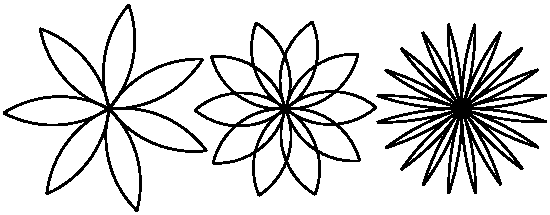
\includegraphics[scale=0.8]{../source/figs/flowers.pdf}}
\caption{Turtle flowers.}
\label{fig.flowers}
\end{figure}

\begin{exercise}
\index{flower}

Write an appropriately general set of functions that
can draw flowers as in Figure~\ref{fig.flowers}.

编写比较通用的一个可以画出像图4-1中那样花朵的函数集。

Solution: \url{http://thinkpython2.com/code/flower.py},
also requires \url{http://thinkpython2.com/code/polygon.py}.

\href{http://thinkpython2.com/code/flower.py}{参考答案},需要使用\href{http://thinkpython2.com/code/polygon.py}{这个模块}。

\end{exercise}



\begin{figure}
\centerline
{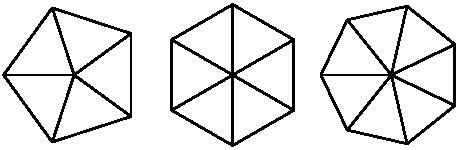
\includegraphics[scale=0.8]{../source/figs/pies.pdf}}
\caption{Turtle pies.}
\label{fig.pies}
\end{figure}


\begin{exercise}
\index{pie}

Write an appropriately general set of functions that
can draw shapes as in Figure~\ref{fig.pies}.

编写比较通用的一个可以画出图4-2中那样图形的函数集,。

Solution: \url{http://thinkpython2.com/code/pie.py}.

\href{http://thinkpython2.com/code/pie.py}{参考答案}

\end{exercise}

\begin{exercise}
\index{alphabet}  \index{turtle typewriter}  \index{typewriter, turtle}

The letters of the alphabet can be constructed from a moderate number
of basic elements, like vertical and horizontal lines and a few
curves.  Design an alphabet that can be drawn with a minimal
number of basic elements and then write functions that draw the letters.

字母表中的字母可以由少量基本元素构成,例如竖线和横线,以及一些曲线。
设计一种可用由最少的基本元素绘制出的字母表,然后编写能画出各个字母的函数。

You should write one function for each letter, with names
\verb"draw_a", \verb"draw_b", etc., and put your functions
in a file named {\tt letters.py}.  You can download a
``turtle typewriter'' from \url{http://thinkpython2.com/code/typewriter.py}
to help you test your code.

你应该为每个字母写一个函数,起名为 \lstinline{draw_a},\lstinline{draw_b} 等等,
然后将你的函数放在一个名为 \lstinline{letters.py} 的文件里。
你可以从 \href{http://thinkpython2.com/code/typewriter.py}{这里}
下载一个``海龟打字员''来帮你测试代码。

You can get a solution from \url{http://thinkpython2.com/code/letters.py};
it also requires \url{http://thinkpython2.com/code/polygon.py}.

你可以在 \href{http://thinkpython2.com/code/letters.py}{这里}找到参考答案;这个解法还要求使用 \href{http://thinkpython2.com/code/polygon.py}{这个模块} 。

\end{exercise}

\begin{exercise}

Read about spirals at \url{http://en.wikipedia.org/wiki/Spiral}; then
write a program that draws an Archimedian spiral (or one of the other
kinds).  Solution: \url{http://thinkpython2.com/code/spiral.py}.

阅读关于 \href{https://zh.wikipedia.org/wiki/%E8%9E%BA%E7%BA%BF}{螺线} (\href{http://en.wikipedia.org/wiki/Spiral}{spiral}) 的相关知识;
然后编写一个绘制阿基米德螺线(或者其他种类的螺线)的程序。
\index{spiral}  \index{Archimedian spiral}

\href{http://thinkpython2.com/code/spiral.py}{参考答案}

\end{exercise}

% SEIKA
% 23 Mar 2016